\chapter{Evolução de Projetos de Software}

Este trabalho visa contribuir diretamente com um software livre, tratando a evolução do mesmo. Dessa forma, neste capítulo, apresentamos os principais conceitos relacionados com esse tipo de software, passando pelas definições básicas, processos de desenvolvimento e os padrões para se contribuir com um projeto de software livre. Complementarmente, discutimos o que é evolução de software, tratando as Leis de Lehman e como está apresentada na literatura os estudos sobre a evolução de projeto de software livre.

%-------------------------------------------------------------------------------

\chapter{Software Livre}

Como este trabalho visa contribuir diretamente com um software livre, neste capítulo serão apresentados os principais conceitos relacionados com esse tipo de software. Em um primeiro momento serão apresentadas definições básicas sobre software livre, já na seção 2.1 processos de desenvolvimento relacionados a esse tipo de software são introduzidos, e finalmente na seção 2.2 são apresentados padrões de software livre.

Um software é constituído por um conjunto de procedimentos, dados, possível documentação, e satisfaz necessidades específicas de determinados usuários. O software é um componente de um sistema computacional de interesse geral, uma vez que vários aspectos relacionados a ele ultrapassam questões técnicas \cite{meirelles2013metrics}, como por exemplo: 

\begin{itemize}
\item O processo de desenvolvimento de software;
\item Os mecanismos econômicos (gerenciais, competitivos, sociais, cognitivos, etc.) que regem esse desenvolvimento e seu uso;
\item O relacionamento entre desenvolvedores, fornecedores e usuários de software;
\item Os aspectos éticos e legais relacionados ao software;
\end{itemize}

%Diferenciar software livre de software proprietario
O entendimento desses quatro pontos é o que diferencia softwares ditos proprietários dos softwares livres, além de definir o que é conhecido como ecossitema do software livre. O princípio básico desse ecossistema é promover a liberdade do usuário, sem discriminar quem tem permissão para usar um software e seus limites de uso, baseado na colaboração e num processo de desenvolvimento aberto \cite{meirelles2013metrics}.

Ao contrário do software proprietário, o software livre tem a característica do compartilhamento do seu código-fonte. Essa característica oferece vantagens em relação ao software proprietário. O compartilhamento permite a simplificação de aplicações personalizadas, já que não necessitam serem codificadas do zero, podendo se basear em soluções existentes. Outra vantagem é a melhoria da qualidade \cite{Raymond, 1999}, por conta da grande quantidade de colaboradores, que com diferentes perspectivas e necessidades, propõem melhorias para o sistema, além de identificar e corrgir bugs com mais rapidez.

Software livre representa uma classe de sistemas de software, os quais são distribuídos sob licenças cujos termos permitem aos seus usuários utilizar, estudar, modificar e redistribuir o software \cite{terceiro2012freesoftware}. 

\section{Processo de Desenvolvimento de Software Livre}

O aspecto mais importante de um software livre, sob a perspectiva da Engenharia de Software é o seu processo de desenvolvimento. Um projeto de software livre começa quando um desenvolvedor individual ou uma organização decidem tornar um projeto de software acessível ao público. Seu código-fonte é licenciado de forma a permitir seu acesso e alterações subsequentes por qualquer pessoa. Tipicamente, qualquer pessoa pode contribuir com o desenvolvimento, mas mantenedores ou líderes decidem quais contribuições serão incorporadas à release oficial. Não é uma regra, mas projetos de software livre, muitas vezes, recebem colaboração de pessoas geograficamente distantes que se organizam ao redor de um ou mais líderes \cite{corbucci2011freemethods}. 

Há características presentes no software livre que, a princípio, tornam incompatível a aplicação de métodos ágeis em seu desenvolvimento. Entre essas características estão a distância entre os desenvolvedores e a diversidade entre suas culturas, que dificultam a comunicação, um dos principais valores dos métodos ágeis. Porém o sucesso resultante de alguns projetos de software livre como é o caso do Kernel do Linux \footnote{\url{https://www.kernel.org/}} fizeram surgir estudos com foco na união dessas duas vertentes.

Analisando um pouco melhor projetos de software livre, é possível notar que esses compartilham princípios e valores presentes no manifesto ágil \footnote{Manifesto Ágil}. Adaptação a mudanças, trabalhar com feedback contínuo, entregar funcionalidades reais, respeitar colaboradores e usuários e enfrentar desafios, são qualidades esperadas em desenvolvedores que utilizam métodos ágeis e são naturalmente encontradas em projetos de software livre.

Num trabalho realizado, Corbucci \cite{corbucci2011freemethods} analisa semelhanças entre projetos de software livre e métodos ágeis através de uma relação entre os quatro valores enunciados no manifesto ágil e práticas realizadas em projetos livres. Abaixo se encontra o texto principal do manifesto:

\begin{mdframed}
"Estamos descobrindo maneiras melhores de desenvolver software, fazendo-o nós mesmos
e ajudando outros a fazerem o mesmo. Através deste trabalho, passamos a valorizar:

\begin{itemize}
\item \textbf{Indivíduos e interações} mais que processos e ferramentas;
\item \textbf{Software em funcionamento} mais que documentação abrangente;
\item \textbf{Colaboração com o cliente} mais que negociação de contratos e
\item \textbf{Responder a mudanças} mais que seguir um plano.
\end{itemize}

Ou seja, mesmo havendo valor nos itens da direita, valorizamos mais os itens da esquerda."
\end{mdframed}

%[Terminar - descrever relação entre valores do manifesto ágil e práticas de projetos de software livre]

\section{Padrões de Software Livre}

Um software livre é concebido através de um processo de contribuições, o qual possui características especiais que promovem o surgimento de diversas práticas influenciadas por diversas forças. Tais práticas são conhecidas como padrões de software livre. Para simplificar, nesta seção o termo padrão está associado a padrões de software livre. Esses padrões estão organizados dentro de três grupos:

\begin{itemize}
\item \textbf{Padrões de seleção} auxiliam prováveis colaboradores a selecionar projetos adequados.
	\begin{itemize}
\item O primeiro padrão de seleção recomenda colaboradores novatos a "caminhar sobre terreno conhecido", ou seja, se deseja contribuir,  começar por algum software que seja familiar, como por exemplo, um browser, editor de texto, IDE\footnote{Integrated Development Environment, um ambiente integrado para desenvolvimento de software}, ou qualquer outro software que já se utiliza.
\item O segundo padrão é similar ao primeiro, porém ao invés da ferramenta ser familiar, esse padrão recomenda que o colaborador tenha conhecimentos na linguagem ou tecnologia utilizada no projeto.
\item Já o terceiro padrão desse grupo motiva colaboradores a procurar por projetos de software livre que ofereçam fucionalidades atrativas, mesmo que o novo colaborador não tenha familiaridade com a ferramenta nem com a tecnologia utilizada em seu desenvolvimento.
\end{itemize}

O terceiro padrão é o que melhor se encaixa ao contexto desse trabalho, já que o Mezuro não era uma ferramenta utilizada no cotidiano e tão pouco familiar. Além disso, as tecnologias utilizadas em seu desenvolvimento não eram as de maior conhecimento. Porém as funcionalidades providas por essa plataforma foi determinante para essa contribuição.

\item \textbf{Padrões de envolvimento} lidam com os primeiros passos para que o colaborador se familiarize e se envolva com o projeto selecionado.
	\begin{itemize}
	\item Entrar em contato com mantenedores para aprender sobre o contexto histórico e político no qual aquele projeto está inserido.
	\item Realizar instalação e checar se todo o ambiente do projeto está corretamente configurado em um período limitado de tempo (máximo um dia)
	\item Durante uma apresentação do sistema,  por parte de algum mantenedor, interagir para se familiarizar melhor com funcionalidades e cenários presentes no sistema.
	\item Avaliar o estado do sistema através de uma breve, mas intensa revisão de código. Isso ajuda a ter uma primeira impressão sobre a qualidade do código-fonte.
	\item Através da leitura, avaliar a relevancia da documentação em um período limitado de tempo.
	\item Checar a lista de tarefas a serem feitas. Ela pode conter bons pontos de partida para começar uma contribuição.
	\item Relacionado ao padrão mencionado acima, está o padrão que recomenda novos colaboradores iniciarem por tarefas mais fáceis. Começar uma tarefa e termina-la é importante para manter colaboradores motivados, e conforme ganharem mais experiencia e familiaridade com o software avançam para tarefas mais complexas.
	\end{itemize}
	No contexto deste trabalho, muitos dos padrões desse grupo foram inseridos ao processo de contribuição, mesmo que incoscientemente. Por exemplo, o orientador deste trabalho e também mantenedor da plataforma Mezuro, assim como outros colaboradores da plataforma, auxiliaram durante o processo de envolvimento, apresentando funcionalidades e principais cenários do sistema, além de fornecer documentação necessaŕia para o entendimento do histórico e contexto no qual o Mezuro está inserido.
	
\item \textbf{Padrões de contribuição} documenta as melhores práticas para se contribuir com softwares livres. Os grupos anteriores tratavam como iniciar e se familiarizar com um projeto de software livre. Esse grupo, por sua vez, contem padrões que auxiliam o fornecimento de insumos para projetos de software livre, seja codigo-fonte ou outros artefatos presentes no processo de desenvolvimento.
	\begin{itemize}
	\item Uma boa contribuição para projetos de software em geral, é a escrita de documentação. O código-fonte muitas vezes não é o suficiente para que todos os envolvidos entendam o andamento do projeto, pois apesar de promoverem o software não possuem conhecimento técnico suficiente. Além disso, documentação do projeto auxilia na manutenção e evolução do produto.
	\item Muitos softwares livres não suportam o idioma de diversos colaboradores. Um bom ponto de partida seria a internacionalização do sistema, incluindo a própria linguagem no sistema.
	\item Reportar bugs eficientemente, pois é comum que colaboradores identifiquem bugs mas ao reporta-los não são claros com respeito ao seu contexto, dificultado sua correção.
	\item Utilizar a versão correta para tarefas. Durante o desenvolvimento de software há diferentes versões, onde há no mínimo uma versão estável e uma versão desenvolvimento. É recomendado utiliar a versão estável para reportar bugs e a versão de desenvolvimento para implementar novas funcionalidades e tudo que não está relacionado com correção de defeitos existentes.
	\item Separar alterações não relacionadas. Se tratando de sistemas de controle de versão\footnote{SCM - Source Code Management - GIT, SVN, Baazar, Mercurial, entre outros} há uma ação conhecida como commit, onde as alterações realizadas são agrupadas e gravadas. É recomendado que num mesmo commit as alterações sejam relacionadas.
	\item Mensagens de commit explicativas para facilitar o entendimento e identificação do que foi desenvolvido ou alterado para o restante dos colaboradores.
	\item Documentar as próprias modificações. Desenvolvedores, geralmente, alteram o código, corrigem bugs, adicionam novas funcioanlidades, mas não atualizam a documentação, a qual se torna desatualizada. Por isso é recomendado documentar as alterações antes de submete-as ao repositório.
	\item Manter-se atualizado com o estado atual do projeto, ajudando a evitar duplicação de esforços e identificar oportunidades de colaboração. Isso é importante pois um projeto de software livre é um esforço coletivo, mas às vezes é difícil coordenar o esforço de pessoas com diferentes horários e prioridades.
	\end{itemize}
\end{itemize}



%Lembrando que esses padrões não são regras, apenas indicam um bom caminho para contribuições. Por exemplo, o software tratado neste trabalho não era familiar no início do processo de contribuição













%-------------------------------------------------------------------------------

\section{Evolução de Software}

Atualmente as tecnologias da informação exercem cada vez mais influência na sociedade, seja na interação entre pessoas, ou nas relações que empresas possuem com o mercado. Empresas, que possuem parte dos seus lucros associados diretamente, ou não, há sistemas de software, precisam evolui-los, seja para adequa-los à mudanças no ambiente onde estão inseridos, ou para mante-los competitivos frente aos concorrentes. Além desses fatores, quando os sistemas em questão são desenvolvidos como softwares livres, eles também precisam evoluir para que se mantenham sempre atrativos, motivando a comunidade estabelecida ao seu redor. Sistemas estagnados desmotivam usuários ou colaboradores, o que significa risco de perda de mercado ou enfraquecimento de um projeto de software livre, já que esses são feitos de colaboradores
%[modificar esse parágrafo com base no artigo challanges_sw_evolution]

Por outro lado, a manutenção desses sistemas é difícil, consome bastante tempo e recursos. Tarefas como adicionar novas funcionalidades, suporte a novos dispositivos de hardware, correção de defeitos, entre outros, se tornam mais difíceis conforme o sistema cresce e envelhece \cite{godfrey2000evolution}.

Acima foram mencionados os termos manutenção e evolução de software. Na maioria das vezes esses palavras aparecem juntas na literatura, e embora se refiram ao mesmo fenômeno, possuem ênfases diferentes. Manutenção é o ato de manter uma entidade num estado de reparo, capacidade ou disponibilidade, prevenindo-a contra falhas, mantendo a satisfação dos envolvidos ao longo do ciclo de vida do software. Já a evolução refere-se a um processo de mudança contínuo de um estado mais baixo, simples ou pior para um estado mais alto, mais complexo e melhor, refletindo a soma de todas as alterações implementadas no sistema.

%evolução de software sempre existiu, porem nao era estudada
A evolução de software foi identificada pela primeira vez no final dos anos 60, embora não denominada evolução até 1969, quando Meir M. Lehman realizou um estudo com a IBM, com a ideia de melhorar a efetividade de programação dessa empresa. Apesar de não ter recebido tanta atenção e pouco impactado nas práticas de desenvolvimento dessa companhia , esse estudo fez surgir um novo campo de pesquisa, a evolução de software.
%\cite{Artigo IBM}.

Durante esses estudos, Lehman formulou as três primeiras, de um total de oito leis, conhecidas atualmente como leis de Lehman. O restante foi formulado em estudos posteriores, conforme a relevancia desse campo aumentava. O conjunto dessas oito leis estão listadas abaixo:
\begin{table}[H]
\begin{center}
    \begin{tabular}{ | l | p{4cm} | p{9cm} |}
    \hline
    Índice (Ano) & Nome & Descrição \\ \hline
    1 (1974) & Mudança contínua & Um software deve ser continuamente adaptado, caso contrário se torna progressivamente menos satisfatório. \\ \hline
    2 (1974) & Complexidade Crescente & À medida que um software é alterado, sua complexidade cresce, a menos que um trabalho seja feito para mantê-la ou diminuí-la. \\ \hline
    3 (1974) & Auto-regulação & O processo de evolução de software é auto-regulado próximo à distribuição normal com relação às medidas dos atributos de produtos e processos. \\ \hline
    4 (1978) & Conservação da estabilidade organizacional & A não ser que mecanismos de retro-alimentação tenham sido ajustados de maneira apropriada, a taxa media de atividade global efetiva num software em evolução tende a ser manter constante durante o tempo de vida do produto. \\ \hline
    5 (1991) & Conservação da Familiaridade & De maneira geral, a taxa de crescimento incremental e taxa crescimento a longo prazo tende a declinar. \\ \hline
    6 (1991) & Crescimento contínuo & O conteúdo funcional de um software deve ser continuamente aumentado durante seu tempo de vida para para manter a satisfação do usuário. \\ \hline
    7 (1996) & Qualidade decrescente & A qualidade do software será entendida como declinante a menos que o software seja rigorosamente adaptado às mudanças no ambiente operacional. \\ \hline
    8 (1971/96) & Sistema de Retro-alimentação & Processos de evolução de software são sistemas de retro-alimentação em múltiplos níves, em múltiplos laços (loops) e envolvendo múltiplos agentes. \\ \hline
    \end{tabular}
    \caption{Leis de Lehman, extraído de \cite{fernandez2008empirical}}
    \label{tab-leis-lehman}
\end{center}
\end{table}

Ao contrário das engenharias tradicionais, a engenharia de software tem em mãos um produto abstrato e intangível, o que resulta em alguns desafios inerentes aos processo de desenvolvimento. A evolução de software busca amenizar ou solucionar alguns desses desafios \cite{mens2005challenges}, entre eles:

\begin{itemize}
\item Manter e melhorar a qualidade do software;
\item Suportar evolução do modelo de desenvolvimento (não só código-fonte);
\item Manter consistência entre artefatos relacionados;
\item Integrar mudanças dentro do ciclo de desenvolvimento de software;
\item Necessidades de bons sistemas de controle de versão;
\item Integração e análise de dados de várias fontes (relatórios de erros, métricas, solicitações de mudança);
\end{itemize}

%importancia
Quando inserida ou considerada nos processos de desenvolvimento ela resulta numa excelente alternativa para evitar os sintomas do envelhecimento e inconsistencias entre o próprio software e o ambinte onde está inserido \cite{mens2005challenges}.

%\subsection{Evolução de Software Livre}

%grande crescimento dos softwares livres em geral, a exemplo do linux
Não restam dúvidas que o desenvolvimento de softwares livres tem produzido softwares de alta qualidade com grande número de funcionalidades. Um exemplo disso é o sistema operacional Linux, que ultimamente tem experimentado um grande sucesso comercial.

Em geral sistemas desenvolvidos por meio de projetos de software livre tendem a crescer com o passar do tempo, após sucessivas releases. Esse comportamento sugere consistência com a sexta lei de Lehman, que se refere ao crescimento contínuo. Nesse sentido, além de um comportamento necessário para manter a satisfação do usuário, o crescimento contínuo de um software livre é importante para manter a motivação da comunidade estabelecida ao seu redor.

Para avaliar esse comportamento de contínuo crescimento em softwares livres Godfray \cite{godfrey2000evolution} e Mockus \cite{mockus2000case}, realizaram pesquisas, do tipo estudo de caso, baseados no sistema operacinal Linux e no servidor de aplicação Apache, respectivamente.

A Figura \ref{Figura1} mostra o crescimento do sistema operacional Linux desde sua primeira release, no ano de 1994. Desde então, ele é mantido por centenas de desenvolvedores que o desenvolvem em dois ramos paralelos: stable releases contendo as principais atualizações e correções de defeitos, e development releases com funcionalidades experimentais e porções de código não testado.

\graphicspath{{figuras/}}
\begin{figure}[H]
\centering
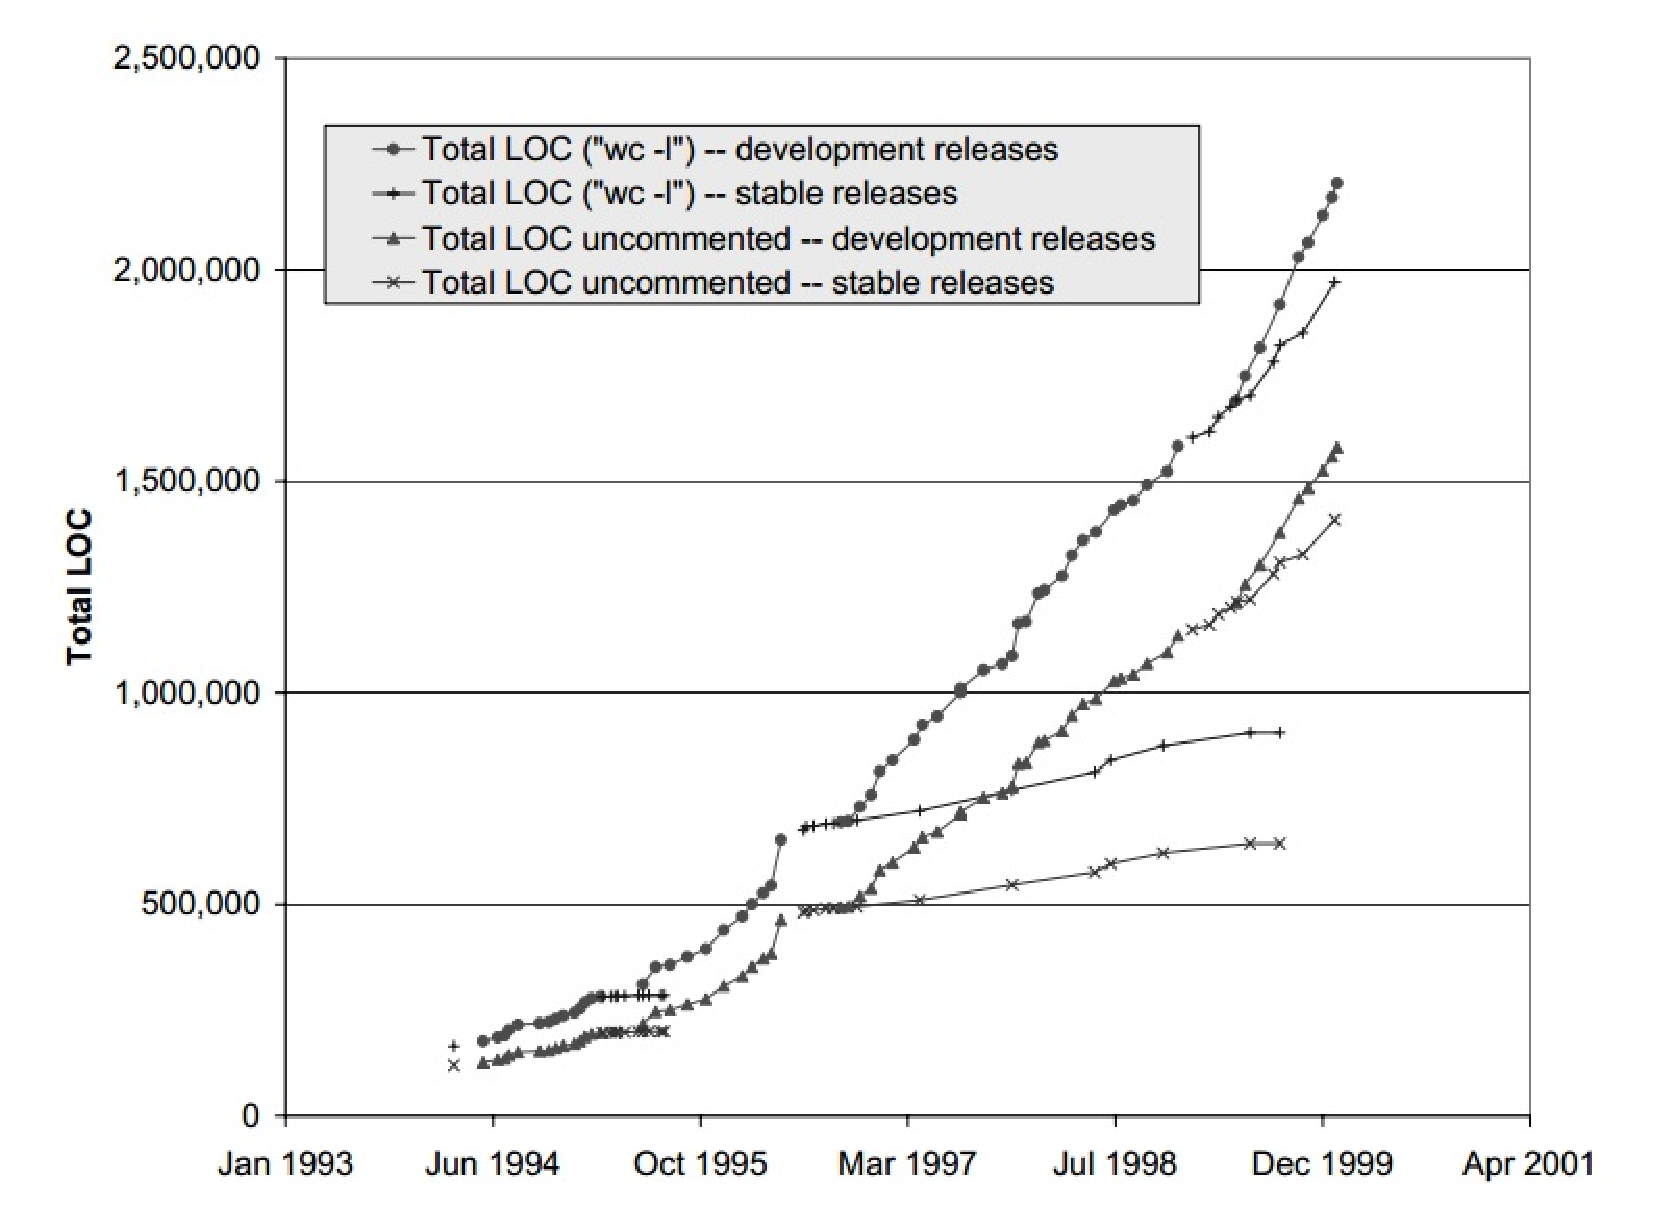
\includegraphics[width=0.6\textwidth]{linux-evolution}
\caption{Evolução do sistema operacional Linux, extraído de \cite{godfrey2000evolution}}
\label{Figura1}
\end{figure}

Os dados presentes no gráfico, até o início dos anos 2000, vão de encontro à quinta lei de Lehman, citada na Tabela \ref{tab-leis-lehman}. No gráfico, o número de linhas de código (LOC) do kernel do sistema, possui taxa de crescimento positiva, enquanto a lei afirma que ao longo do tempo a taxa de crescimento tende a diminuir.%Lehman e Turski tinham a hipótese da taxa do quadrado inverso do crescimento ao longo do tempo.









